\chapter{YaST2.call}

YaST2.call works in the First-Stage environment as well as in the
Second-Stage environment. The YaST2.call script includes all the tasks
which needs to be handled independent of the environment. YaST2.call
requires a correct prepared environment done within the YaST2-First-Stage
or YaST2-Second-Stage scripts. Its major task is to start YaST2.
The following workflow shows how YaST2.call works.

\begin{figure}[h]
\caption{Run Workflow}
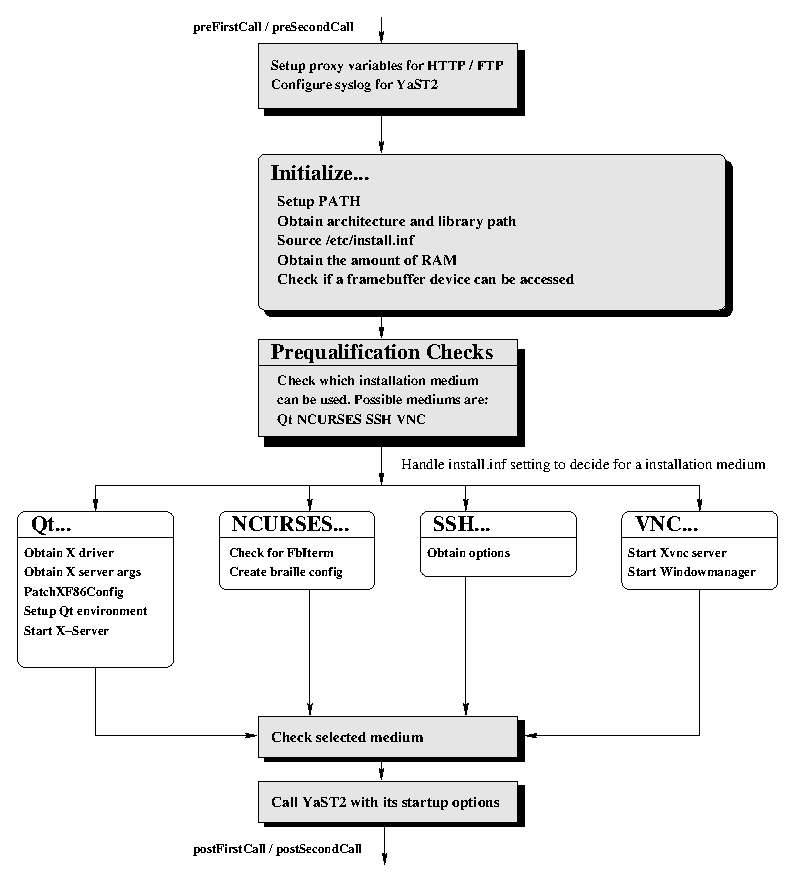
\includegraphics[scale=1]{pictures/run.eps}
\end{figure}

\section{Call-Stage Hooks}
The following Call-Stage hook directories are checked:

\begin{itemize}
\item \textbf{\underline{preFirstCall}}\\
	Within the inst-sys each script stored in the preFirstCall directory is
	called directly in front of the YaST2.call script
\item \textbf{\underline{postFirstCall}}\\
	Within the ins-sys each script stored in the postFirstCall directory is
	called directly after the YaST2.call script has been finished
\item \textbf{\underline{preSecondCall}}\\
	Within the installed system each script stored in the preSecondCall
	directory is called directly in front of the the YaST2.call script
\item \textbf{\underline{postSecondCall}}\\
	Within the installed system each script stored in the postSecondCall
	directory is called directly after the YaST2.call script has been
	finished
\end{itemize}

\section{Medium prequalification}
There are four different mediums to use for an installation. Each
of them have a view needs which should be checked first to know
about the possible mediums to use.

\begin{itemize}
\item Qt
	\begin{enumerate}
	\item Qt plugins are needed
	\item Appropriate X driver module must be found
	\item Memory requirements must be fulfilled
	\item X-Server needs to be started if there is no DISPLAY to access either
	\item /etc/X11/xorg.conf must exist
	\item /usr/X11R6/share/fvwm/fvwmrc.yast2 must exist
	\end{enumerate}
\item NCURSES\\
	There are no prerequires for ncurses mode
\item SSH
	\begin{enumerate}
	\item sshd must be running
	\end{enumerate}
\item VNC
	\begin{enumerate}
	\item /usr/X11R6/share/fvwm/fvwmrc.yast2 must exist
	\end{enumerate}
\end{itemize}


\section{Medium selection check and fallback}
The default medium is Qt but the medium can be changed with options
given to the bootmanager. The options are passed to the kernel, linuxrc
will handle it and provide the options not handled within the
file \textbf{/etc/install.inf}. Refering this information one of the
possible mediums is selected. If the medium cannot be selected because
of a missing prerequirement the NCURSES fallback is used.

If the prequirements for the selected medium is ok we will handle the
installation medium according to the workflow above. After the medium
has been prepared we need to check the medium again:

\begin{itemize}
\item Qt
	\begin{enumerate}
	\item If an X-Server must be started, check if the server is running and
          accessable
	\end{enumerate}
\item NCURSES\\
    There are no checks for the ncurses mode
\item SSH
    \begin{enumerate}
    \item The network interface has to be reachable
    \end{enumerate}
\item VNC
    \begin{enumerate}
    \item The Xvnc server must be running
    \end{enumerate}
\end{itemize}

If one of the medium selection checks failed this should be handled as
a fatal error and should be shown in a descriptive error message.
